\chapter{Related Work}

The need to understand human measurements has always been essential. The methods for obtaining these measurements have continually evolved, and today, they rival traditional techniques in precision. This progress has been driven by innovative ways of collecting data for these estimations.

%The solution proposed in \cite{HBDE1} provides us with a method which estimates subject's height using single uncalibrated image. Another approach  \cite{KeepItSMPL} uses joints position estimation to create a 3D mesh used for further evaluation.
\section{History of Anthropometry}
Quetelet's concept of the "average man"~\cite{QUETELET} has profoundly influenced the development of psychology and the statistical study of human characteristics. Quetelet argued that measurements of human traits would conform to a normal distribution, with the average representing the true or ideal type. This notion of the average as representative allowed early psychologists to blur the distinction between individual-level data and aggregate statistics. Success of this idea cannot be diminished as one of the outcomes of this the idea Body Mass Index (BMI) is still used to this day~\cite{bmiUsage}. The idea of the average man as a statistical model for understanding human nature persisted in psychology, even as reporting practices shifted towards aggregate statistics. Quetelet's work laid the groundwork for the widespread use of large-scale data collection and analysis techniques, which became central to understanding individual differences and population-level phenomena. 

The legacy of Quetelet's work highlights the important epistemic challenges that arise when connecting statistical models to claims about individuals and human nature. This historical context is relevant for understanding the development of methods for estimating human body measurements from data, which often rely on aggregate statistics and population-level modeling.

Another significant impact of anthropometry on human society is illustrated by the Bertillon system~\cite{sus}. In the late 1870s, the French policeman Alphonse Bertillon began measuring prisoners for later identification. This approach helped in identifying recidivists and provided the police with additional information.

In the early 20th century, anthropometric measurements took on a new function. Predictions of body fat were based on measurements such as body length, circumference, and skinfold thickness~\cite{anthroHist2}. This method spread rapidly due to its non-invasiveness, portability, and cost-effectiveness.

Nowadays, anthropometric measurements remain important in multiple fields. Digital anthropometry is being used to measure the size of infants' bodies to check for nutrition and growth anomalies~\cite{nutrition}. Additionally, companies like Treedy's~\cite{treedys} are incorporating digital measuring stations in clothing stores to help customers pick the correct clothing size and even recommend fitting pieces.

\begin{figure}
	\centering{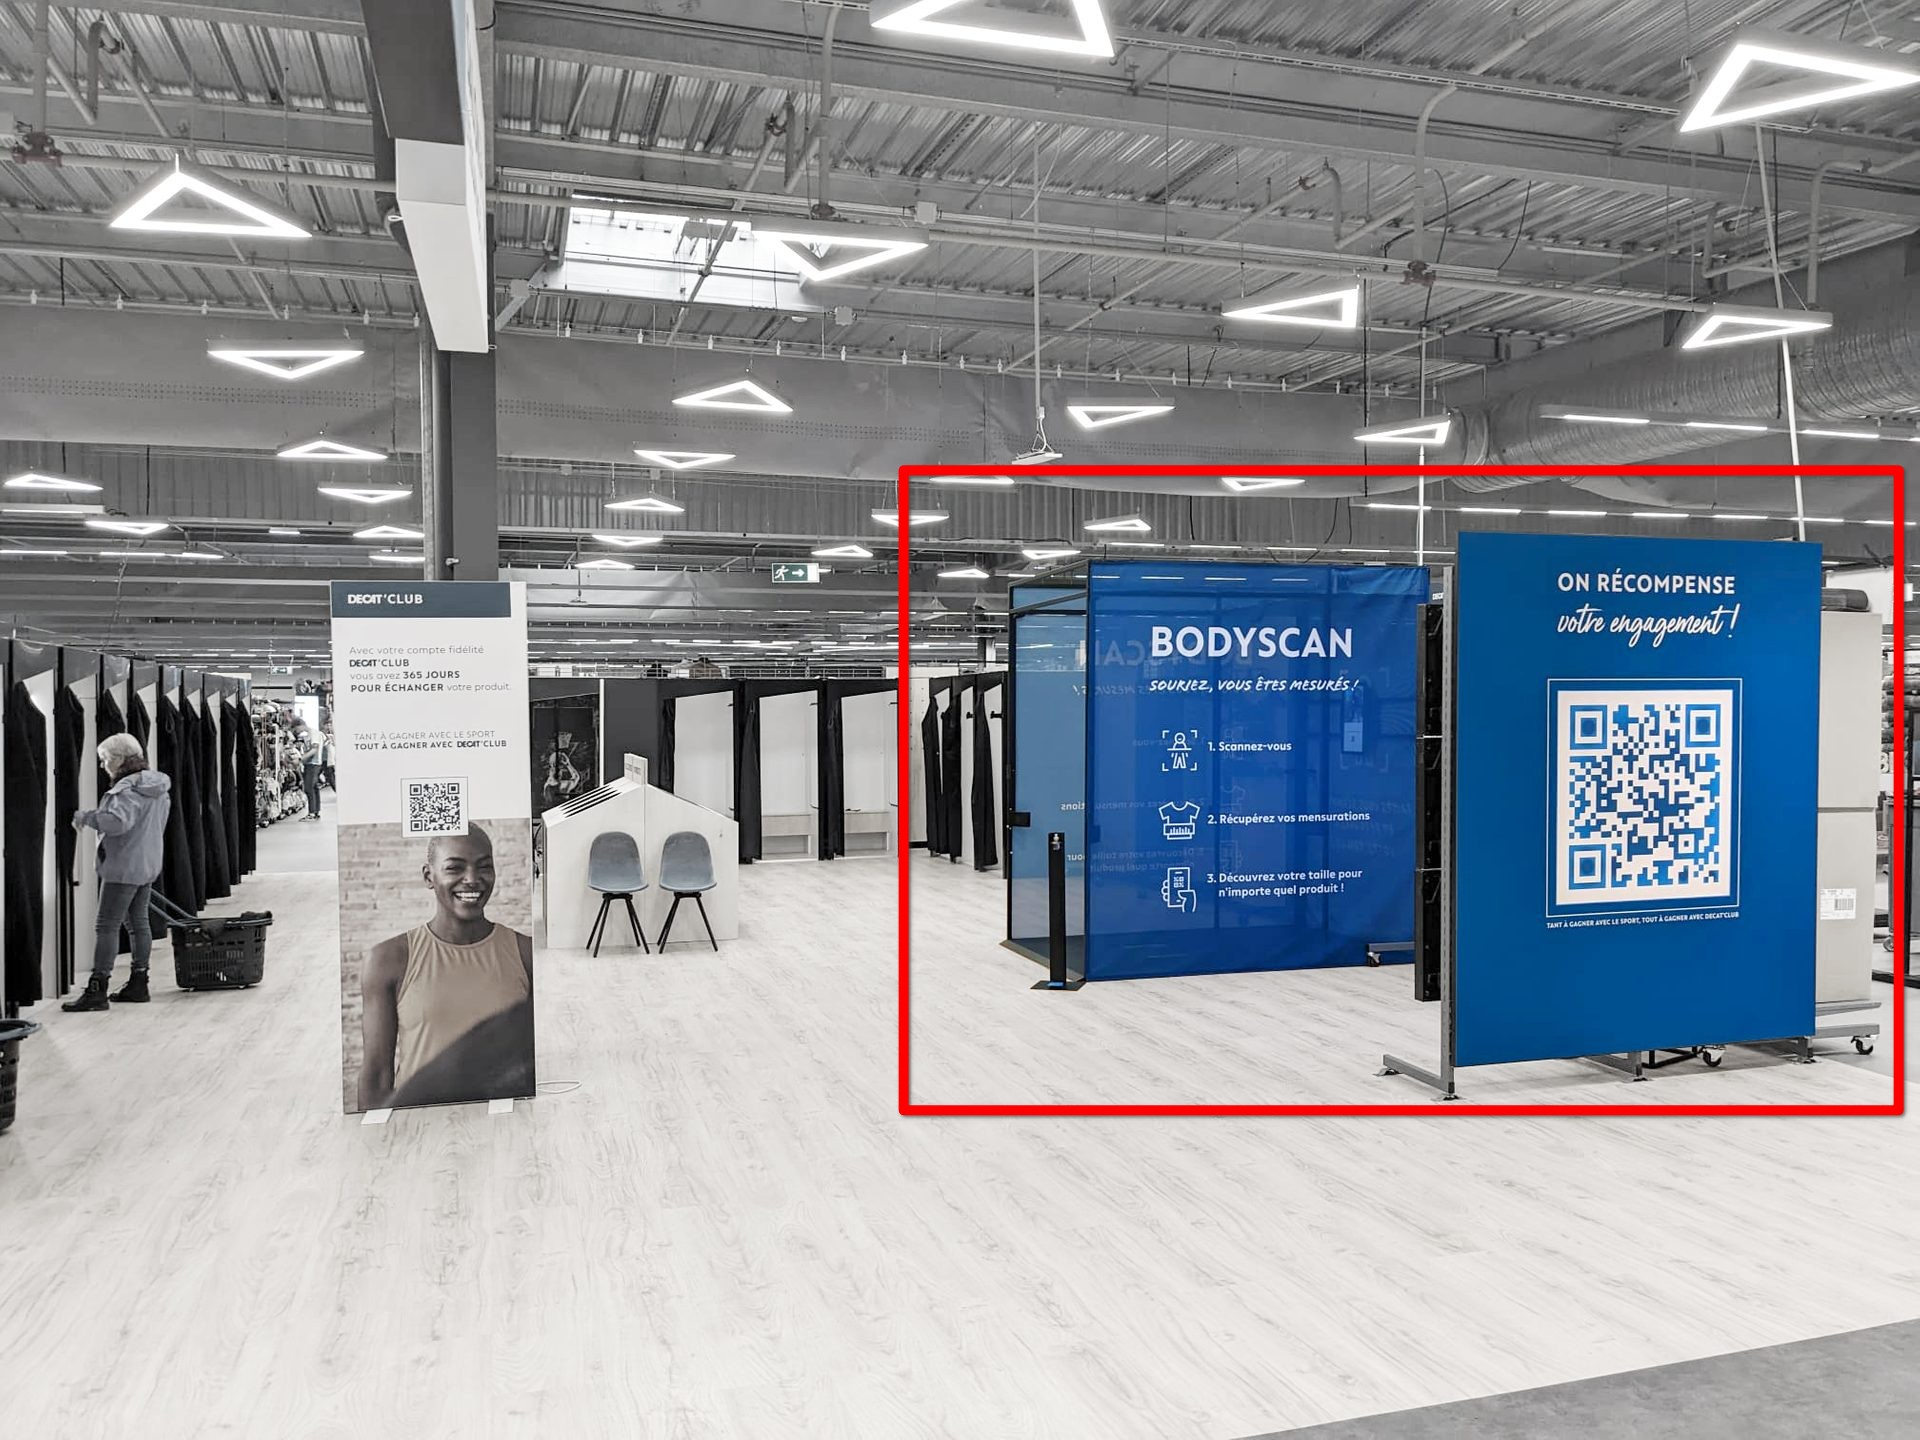
\includegraphics[scale=0.25]{images/Treedys}}
	\caption[Treedy's scanning device]{Treedy's body scanning station used in Decathlon stores. Customers can obtain their body measurements just by walking in. The device scans them using four camera-equipped devices and, using their patented Nakednet AI, estimates the measurements. Credit: Treedy's~\cite{treedys}.}
	\label{treedys}
\end{figure}

\section{Types of Human Body Estimations}
\subsection{Mathematical Models}
The task of calculating the Body Mass Index (BMI) from body dimensions~\cite{bmiPredict} became important in tracking the development of pandemic of obesity during the 20th century~\cite{bmiUsage}. This has enabled researchers to create statistical models to detect overweight or underweight conditions in the population. The measurements required for these tasks varied, but the popular approach resulted in requiring only height and weight~\cite{bmiHW} based on the BMI formula~\cite{bmi}.

Another task was the determination of the centre of mass of the human body, the moment of inertia, and their products, including BMI. These parameters were necessary for various applications, such as Self-Maneuvering Units~\cite{bodyInertia} used for extravehicular movement in space or the development of prosthetic devices and man-machine interfaces~\cite{bodyInertia2}. These tasks continue to be researched today~\cite{bodyMotion}, highlighting the ongoing need for such studies.

In anthropology, an anatomical task arose to estimate human stature from parts of the skeleton~\cite{skeletonHeight}. Researchers have used different indicators such as brain weight~\cite{brainStature}, femur size~\cite{femurStature}, and many more~\cite{statureHistory} to estimate the stature. This information aids scientists to understand the shape, evolution, and environmental influences on humanity.
\subsection{Regression}
As powerful computational devices became available to scientists, the more complex models of regression analysis has enabled more precise estimations than the aforementioned approaches. Over the years the popularity of regression grew not only for precision of results, but also thanks to the ubiquity and availability  of large amounts of data~\cite{regressionStature}. In recent years it has became an essential part of statistics for students of anthropology~\cite{regressionStudents}.

The methods used for regression are often not much different to the mathematical models, based on the same hypotheses. 
Important research was done by Trotter and Gleser~\cite{regressionBig}, who used regression to estimate relationship between different bone lengths and stature. Providing study based on large dataset with newly addressed aging factor and bringing groundbreaking results~\cite{statureComparisons}.

Regression is often used in cases when it was unable to recover all parts of human skeleton~\cite{regressionBulk} to perform traditional forensic methods. For example the hand length~\cite{regressionHandFoot, regressionHand} (or more recently~\cite{handNew, handNew2}) or foot~\cite{regressionHandFoot,regressionFoot} are plausible to use. Moreover, the regression can be used for predicting whole-body fat mass, lean mass and trunk fat mass~\cite{regressionBodyFat}. These regression equations used BMI, WC, gender and age to provide results. 

\subsection{Images}

In more recent years the approach to use image data to estimate stature has been introduced. The images can be calibrated or uncalibrated~\cite{estimationImages, image}. While the scale of calibrated image can be calculated with knowledge, the uncalibrated image is a more complex process. Usually there would be a need for a reference length, but this article obviates the need thanks to use of statistical height of humans. Mentioned methods and other methods~\cite{image2}, do not however primarily focus on anthropometric measurements, yet they usually use stature for different tasks. 

A possible solution to our task is presented by Meunier et. al.~\cite{image2DMeasurements}. Mentioned approach is based on taking pictures from two calibrated cameras and finding landmarks on the subject. The circumferences cannot be measured directly and have to be estimated using mathematical models. A different approach suggested by Hung et. al.~\cite{image2DMeasurements2}, uses a single camera and a calibration square to take three pictures (front, side, back). Moreover, the circumferences were not estimated using a mathematical model, but by estimating shape from multiple images.  Another, more recent approach uses five images and a linear regression to estimate the measurements, but uses manual annotation of the landmarks on the subject~\cite{images}. Very simple and cheap approach uses just one webcamera and A4 sheet of paper in multiple pictures of a person. The A4 paper is then used as a scale for Pixel Density Method to estimate dimensions.

\subsection{Virtual Representation}
Another step in anthropometry was brought by usage of 3D data. These are usually collected by special devices that provide extra information over usual cameras (see Section \ref{3Ddata} for more information). After all necessary data is captured, a processing algorithm (such as Iterative Closest Point~\cite{pointcloudProcess}) is run to unify data from multiple images and as result generates a point cloud or a 3D mesh~\cite{digitalAnthro}. These structures are proficient in providing the necessary means to calculate the required measurements. The measuring process can be done manually~\cite{3Dextraction}, providing the user with measurements at selected points, or by automatic landmark locating. Approach suggested by Tomi et. al.~\cite{kinect} uses angle-based algorithm to calculate the width and thickness of subject's body. Then, using joint information provided by capturing device's (Kinect) SDK, finds the leftmost and rightmost points of given measurement and calculate the distance between them. For circumferences, they use ellipse perimeter equation. Different approach uses a deep neural network to extract required measurements~\cite{pointcloudNN}. This approach is based upon a template on which the measuring points are defined. The network takes the template and deforms it to look like the input. The output of this network is a deformed template with measuring points, that can be measured with point-to-point distance.


\section{Domain Adaptation}
When training a machine learning model, such as a neural network, it is crucial for the performance of the model that the training and testing data are similar and follow the same distribution~\cite{domainAdaptation}. However, this condition is often not met. One reason for this is the limited amount of training data, as demonstrated in this thesis. Another reason is the slight differences between the test data and the data the network was trained on. For instance, this can occur with medical devices where output devices may have varying colour representations. Considering factors like time complexity and data availability, domain adaptation can be an optimal solution to address these discrepancies.

Domain adaptation is a type of transfer learning, used to mitigate domain shift between source (training data) and target (data used for testing) domain~\cite{domainAdaptation}.
The assumption behind domain adaptation is, that there exists a difference in domains (source and target), but not in the task. Furthermore, the domains should not be too different and should have similar probability distributions. These limitations impact the performance, up to point where network's performance may be worse than before applying domain adaptation if used incorrectly. On the other hand, there are multiple advantages to using domain adaptation. For example, the cost of collecting and labelling new data can be mitigated. In addition, the resulting network is able to generalise better on the target domain. Multiple domain adaptation approaches have been developed to address this issue~\cite{domainAdaptationGod}.

\subsection{Instance Re-weighting Methods}
\label{Instance}
  Instance re-weighting aims to mitigate the issue of sample selection bias by assigning different weights to source domain instances based on their relevance to the target domain distribution. Sample selection bias occurs when the samples selected for model training are not representative of the population or the conditions that the model will encounter.  This bias can lead to skewed or incorrect conclusions. One of the notable approaches, Kernel Mean Matching~\cite{instanceMethod} (or KMM for short),  aims to adjust the distribution of the source domain by assigning weights to source instances. 
 
 \subsection{Feature Adaptation Methods}
 \label{Feature}
 Feature-based methods focus on finding a common feature representation that is invariant across domains. These methods typically involve transforming the feature space such that the source and target domains become indistinguishable. One important method is the Maximum Mean Discrepancy (MMD). DAN~\cite{featureMethod} incorporates MMD into a deep neural network, aligning the distributions of source and target features at multiple layers of the network. %Explain MMD
 
 Another influential method is Domain-Adversarial Neural Networks (DANN)~\cite{featureMethod2}. DANN employs adversarial training, where a domain classifier is trained to be able to distinguish source and target features while the feature extractor simultaneously learns to confuse the domain classifier. This adversarial process influences the feature extractor to generate domain-invariant features, enhancing model performance on the target domain.
 
\subsection{Classifier Adaptation Methods}
\label{Classifier}
Classifier adaptation methods aim to develop a general classifier by utilizing labeled samples from the source domain along with a few labeled samples from the target domain.

ASVM~\cite{asvm} is an example of kernel classifier-based methods. It adjusts the decision boundary learned from the source domain to fit the target domain by adding a bias function $\Delta f(x)$ to the source classifier. This bias function is parameterized by $w$ and optimized using SVM techniques to minimize classification errors on the target domain data. 
 
 \subsection{Deep Network Adaptation Methods}
Deep network adaptation is a prominent technique in domain adaptation, leveraging the powerful feature representation and end-to-end training capabilities of deep neural networks. The methods mentioned so far can be used in deep neural networks


\subsection{Adversarial Adaptation Methods}
This approach focuses on minimizing domain discrepancies by training models to generate domain-invariant features or pixel-level target samples. CyCADA (Cycle-Consistent Adversarial Domain Adaptation)~\cite{hybridMethod} combines adversarial training, cycle-consistency, and feature alignment. CyCADA uses generative adversarial networks (GANs) to generate images from domains. This approach helps align the feature distributions while preserving the semantic content, leading to improved adaptation performance.

CyCADA uses principles proposed by CycleGAN~\cite{CycleGAN}. Firstly, it employs a generators and discriminators to create cycle consistency. The generators are used to map images from the source domain to the target domain and then back to the original domain. The difference between input image and the image transformed back to source domain is used as a loss called cycle-consistency loss. The whole loss is then created by summing the cycle consistency loss and two generator losses.


\section{Data Acquisition}
Neural networks have caused a shift in task solving in numerous fields. The tasks, which can be neural networks used for are rather complex and require a large amount of carefully prepared datasets. To create such dataset, the data has to be collected and further correctly labelled. There are, however, many obstacles that have to be overcome to create usable dataset, of which some are:

\paragraph{Cost} Creating datasets can be expensive as they have to be large, often requiring multiple workers to collect and label data. In some cases special devices and environment may be required to be able to obtain such data, which further increases the cost.
\paragraph{Time} As the type of data vary from task to task, the data may be complicated to obtain, such as taking photographs in different regions or measuring values using complex machinery or many others. The data collection is, however, only half of the task. The other half consists of correctly labelling the data. Depending upon the task, it can sometimes require professionals to assess the data.
\paragraph{Privacy} In many medical applications the task requires personal data to make correct predictions. This raises concerns about private information leaking and thus the data has to be dealt with in way it follows all privacy regulations. Moreover, there must be enough willing patients to be able to procure such dataset, which can raise the monetary cost of such dataset. Medicine is not the only field in which personal information may be required to create suitable dataset.
\paragraph{Robustness} In order for the network to be able to correctly generalise, the dataset should be as general as is possible, including extreme and unusual cases as well. If this is not the case, the network may struggle with such cases or can develop a bias to the most common example. This is often the most complicated task, and it is rarely able to fully contain the whole spectrum.
\paragraph{Availability} Not all data is available all the time and thus obtaining can be impossible at that specific time. Most commonly this issue rises when the subject of the dataset is rare (for example certain illnesses or animals etc.) or is currently not available (wrong season or not appropriate conditions).

\subsection{Synthetic Data}
To overcome these obstacles, some data can be created synthetically. This type of data is artificially generated instead of collected manually. The generation is based on models and algorithms which aim to create samples that are adjusted to meet specific requirements, but also contain features and variation the real data may be missing. The main aim of this data is to make the network more robust, helping it to be precise even in situations that were not included in the real data \cite{synthDataRobust}. Other than better precision, generating data can be far less expensive than collecting it. 

There are currently multiple approaches that are used for generation of synthetic data~\cite{synthDataReview}. 

\section{BMnet}
BMnet~\cite{BodyM} is a network based on MnasNet~\cite{mnasnet}, which is a convolutional neural network.  As an input it requires a frontal silhouette and optionally works with lateral silhouette as well. The lateral silhouettes provide additional information for chest and waist measurements. Moreover, the paper uses height and weight as an input metadata. The height is necessary in situations where the subjects have variable distance to camera making the scale of the subjects non-uniform. Weight then provides yet another information of the subject's size and shape. In the network the images are concatenated spatially, whilst the height and weight are concatenated depth-wise. This object is then evaluated by the MnasNet followed by MLP, consisting of 128 neurons and 14 outputs, providing the results.
The adversarial body simulation (ABS) presented in BMnet work with SMPL~\cite{smpl} model (see Section \ref{smpl}) . Its main goal is to find body shapes that are challenging for BMnet, since they are not as common or even non-existent in the dataset.
 

\section{Neural Anthropometer}
An important article is by Tejeda and Mayer~\cite{source} which proposes a method to tackle the task of estimating anthropometric measurements. The Neural Anthropometer provides a valuable approach. To keep the network as small as possible due to resource consumption and training difficulty increase with size. The proposed architecture starts with a binary image silhouette input. This is then processed by a convolutional layer. Number of channels was based on number of values on output. 

This approach is further implemented by~\cite{super}. The article further delves into different data representations of human bodies and their performance.  
